\section{Randomized PROPAGATION}
\label{sec:RPA}

% \begin{quote}
% 	{\em "Is there a more general way to introduce randomization into graph propagation and reduce the time complexity?"}
% %	, like the $O(m \cdot \log \frac{1}{\lmd})$-bound of $\powitr$?}
% \end{quote}


\header{\bf A failed attempt: pruned propagation.}
The $O\left(m \log \frac{1}{\delta}\right)$ running time is undesirable in many applications. To improve the scalability of the basic propagation algorithm, a simple idea is to prune the nodes with small residues in each iteration. This approach has been widely adapted in local clustering methods such as Nibble and PageRank-Nibble~\cite{FOCS06_FS}. In general, there are two schemes to prune the nodes: 1) we can ignore a node $u$ if its  residue $\hat{\vec{r}}^{(i)}(u)$ is smaller than some threshold $\varepsilon$ in line 3 of Algorithm~\ref{alg:AGP-deter}, or 2) in line 4 of Algorithm~\ref{alg:AGP-deter}, we can somehow ignore an edge $(u,v)$ if $\left(\frac{Y_{i+1}}{Y_i} \right) \cdot \frac{\vec{r}^{(i)}(u)}{d_v^{a} \cdot d_u^b}$, the  residue to be propagated from  
$u$ to $v$, is smaller than some  threshold $\varepsilon'$.  Intuitively, both pruning schemes can reduce the number of operations in each iteration.



However, as it turns out, the two approaches suffer from either unbounded error or large time cost. More specifically, consider the toy graph shown in Figure~\ref{fig:special-case}, on which the goal is to estimate $\vec{\pi}=\left(\mathbf{A}\mathbf{D}^{-1} \right)^2 \cdot \vec{e}_s $, the transition probability vector of a 2-step random walk from node $s$. It is easy to see that $\vec{\pi}(v)=1/2, \vec{\pi}(s) = 1/2$, and $\vec{\pi}(u_i)=0, i=1,\ldots, n$. 
%We focus on the approximation quality of $\vec{\pi}(v)$. In particular, we set $\delta = 1/4$ so that the approximate propagation algorithm has to return a constant approximation of $\vec{\pi}(v)$. 
We focus on constant relative error threshold of $\vec{\pi}(v)$'s approximation (e.g. $\delta = 1/4$). Hence, the approximate propagation algorithm has to return a constant approximation of $\vec{\pi}(v)$. 
\begin{figure}[t]%[h]
	\begin{small}
		\centering
		%\vspace{-4mm}
		%    \begin{footnotesize}
		\begin{tabular}{c}
			%\multicolumn{4}{c}{\hspace{-4mm} \includegraphics[height=5mm]{./Figs/legend_large.eps}} \vspace{-1mm} \\
			%\hspace{-3mm} 
			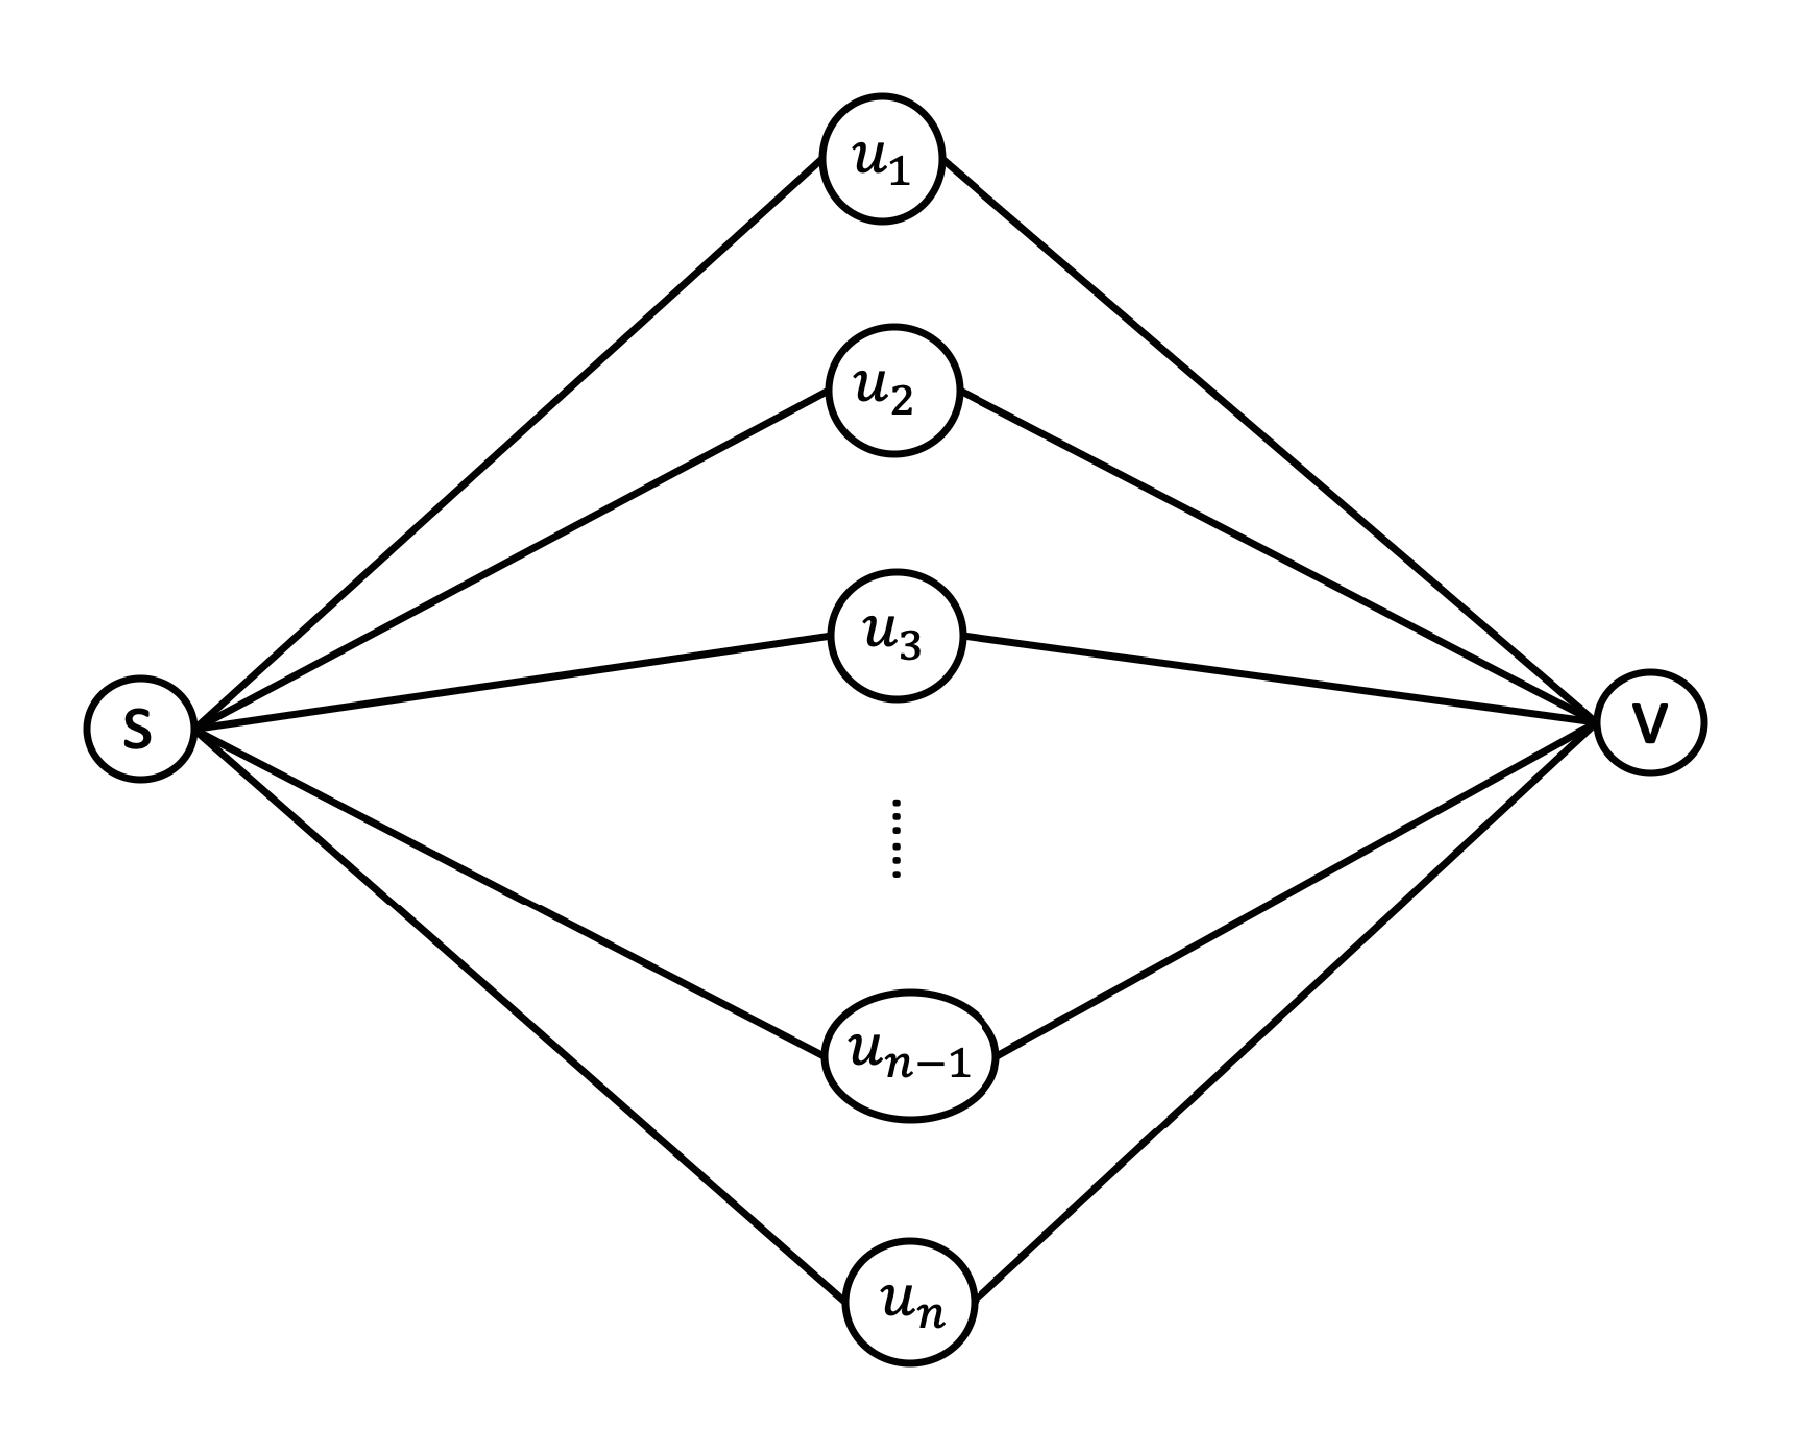
\includegraphics[height=40mm]{./Figs/img_special-case.eps} 
		\end{tabular}
		\vspace{-5mm}
		\caption{A bad-case graph for pruned propagation.} 
		\label{fig:special-case}
		\vspace{-5mm}
	\end{small}
	\vspace{-2mm}
\end{figure}
We consider the first iteration, which pushes the residue $\vec{r}^{(0)}(s)=1$ to $u_1, \ldots, u_n$. If we adopt the first pruning scheme that performs push on $s$ when the residue is large, then we will have to visit all $n$ neighbors of $s$, leading to an intolerable time cost of $O(n)$. On the other hand, we observe that the residue transforms from $s$ to any neighbor $u_i$ is $ \frac{\vec{r}^{(0)}(s)}{d_s} = \frac{1}{n}$. Therefore, if we adopt the second pruning scheme which only performs pushes on edges with large residues to be transformed to, we will simply ignore all pushes from $s$ to $u_1, \ldots, u_n$ and make the incorrect estimation that $\hat{\vec{\pi}}(v)=0$. The problem becomes worse when we are dealing with the general graph propagation equation~\eqref{eqn:pi_gen}, where the Laplacian parameters $a$ and $b$ in the transition matrix $\mathbf{D}^{-a} \mathbf{A}  \mathbf{D}^{-b}$ may take arbitrary values. For example, to the best of our knowledge, no sub-linear approximate algorithm exists for Katz index where $a=b=0$.


% Consequently, a natural question arises: {\em is there a more general way to introduce randomization into graph propagation and reduce the time complexity?}

% In the specific application of estimating the transition probability vector, the above dilemma can be solved by the Monte Carlo method, which simulates a number of 2-step-random-walks from $s$ and uses the percentage of random walks that reaches $v$ as an estimator of $\pi(v)$. The standard probabilistic analysis shows that one only needs to simulate a constant number of random walks to obtain a constant approximation of $\pi(v)$. Therefore, by introducing randomization into the propagation, we can bring the time complexity from $O(n)$ to $O(1)$ and still make the correct estimation with high probability. However, the Monte Carlo method requires that the propagation matrix to be $\mathbf{A} \cdot \mathbf{D}^{-1}$, which is merely a special case of the general graph propagation. Consequently, a natural question arises: is there a more general way to introduce randomization into graph propagation and reduce the time complexity?






%\vspace{-1mm}
%\subsection{Randomized propagation} 
\header{\bf Randomized propagation.} We solve the above dilemma by presenting a simple {\em randomized} propagation algorithm that achieves both theoretical approximation guarantee and near-optimal running time complexity. Algorithm~\ref{alg:AGP-RQ} illustrates the pseudo-code of the Randomized Propagation Algorithm, which only differs from Algorithm~\ref{alg:AGP-deter} by a few lines (4-9). Similar to Algorithm~\ref{alg:AGP-deter},  Algorithm~\ref{alg:AGP-RQ} takes in an undirected graph $G=(V,E)$, a graph signal vector $\vec{x}$, a level number $L$ and a weighted sequence $w_i$ for $i\in [0,L]$. In addition, Algorithm~\ref{alg:AGP-RQ}  takes in an extra parameter $\varepsilon$, which specifies the relative error guarantee. As we shall see in the analysis, $\varepsilon$ is roughly of  the same order as the relative error threshold $\delta$ in Definition~\ref{def:pro-relative}. Similar to Algorithm~\ref{alg:AGP-deter}, we start with $\vec{\hat{r}}^{(0)} = \vec{x}$ and iteratively perform propagation through level 0 to level $L$. The key difference is that, on a node $u$ with non-zero residue $\hat{\vec{r}}^{(i)}(u)$, instead of pushing the residue to the whole neighbor set $N_u$, we only perform pushes to neighbor $v$ with small degree $d_v$. More specifically, for each neighbor $v\in N(u)$ with degree $d_v \le \left( \frac{1}{\varepsilon} \cdot\frac{Y_{i+1}}{Y_i} \cdot \frac{\hat{\vec{r}}^{(i)}(u)}{d_u^b}\right)^{1/a}$, we increase $v$'s residue by $\frac{Y_{i+1}}{Y_i} \cdot \frac{\hat{\vec{{r}}}^{(i)}(u)}{d_v^a\cdot d_u^b}$, which is the same value as in Algorithm~\ref{alg:AGP-deter}. We also note that the condition  $d_v \le \left( \frac{1}{\varepsilon} \cdot\frac{Y_{i+1}}{Y_i} \cdot \frac{\hat{\vec{r}}^{(i)}(u)}{d_u^b}\right)^{1/a}$ is equivalent to $ \frac{Y_{i+1}}{Y_i} \cdot \frac{\hat{\vec{{r}}}^{(i)}(u)}{d_v^a\cdot d_u^b} > \varepsilon$, which means we push the residue from $u$ to $v$ only if it is larger than $\varepsilon$. For the remaining nodes in $N_u$, we sample each neighbor $v\in N_u$ with probability $p_v= \frac{1}{\varepsilon}\cdot \frac{Y_{i+1}}{Y_i}\cdot \frac{\hat{\vec{r}}^{(i)}(u)}{d_v^a\cdot d_u^b}$. Once a node $v$ is sampled, we increase the residue of $v$ by $\varepsilon$. The choice of $p_v$ is to ensure that $p_v\cdot \varepsilon$, the expected residue increment of $v$, equals to $\frac{Y_{i+1}}{Y_i} \cdot \frac{\hat{\vec{r}}^{(i)}(u)}{d_v^a\cdot d_u^b}$, the true residue increment if we perform the actual propagation from $u$ to $v$ in  Algorithm~\ref{alg:AGP-deter}. 


\begin{algorithm}[t]
	\caption{Randomized Propagation Algorithm\label{alg:AGP-RQ}}
	\KwIn{undirected graph $G=(V,E)$, graph signal vector $\vec{x}$ with $\|\vec{x}\|_1 \le 1$, weighted sequence $w_i(i=0,1,...,L)$, error parameter $\varepsilon$, number of levels $L$\\}
	\KwOut{the estimated propagation vector $\hat{\vec{\pi}}$\\}
	%$L\gets \log{\frac{1}{\varepsilon}}$\;
	%$\vec{\hat{r}}^{(i)} \gets \vec{0}$, $\vec{\hat{q}}^{(i)} \gets \vec{0}$, for $i=0,1,...,L$\;
	$\vec{\hat{r}}^{(0)} \gets \vec{x}$\;
	%$\hat{\pi} \gets w_0\cdot \hat{P}^{(0)}$\;
	\For{$i=0$ to $L-1$}{
		\For{each $u \in V$ with non-zero residue $\hat{\vec{r}}^{(i)}(u)$}{
			\For{each $v\in N_u$ and $d_v \hspace{-0.5mm} \le \hspace{-0.5mm} \left(\frac{1}{\varepsilon} \cdot\frac{Y_{i+1}}{Y_i} \cdot \frac{\hat{\vec{r}}^{(i)}(u)}{d_u^b}\right)^{\frac{1}{a}}$}{
				$\vec{\hat{r}}^{(i+1)}(v) \gets \vec{\hat{r}}^{(i+1)}(v)+ \frac{Y_{i+1}}{Y_i} \cdot \frac{\hat{\vec{r}}^{(i)}(u)}{d_v^a\cdot d_u^b} $;
			}
			%$ran \gets rand(0,1)$\;
			%\For{each $v\in N(u)$ and $\frac{\hat{R}^{(i)}(u)}{\varepsilon} \cdot \left( 1- \frac{w_i}{Y_i}\right) < d^{1-r}_v\cdot d^r_u \le \frac{\hat{R}^{(i)}(u)}{ran \cdot \varepsilon} \cdot \left( 1- \frac{w_i}{Y_i}\right)$ }{
			{\bf Subset Sampling}: Sample each remaining neighbor $v\in N_u$ with probability $p_v = \frac{1}{\varepsilon}\cdot \frac{Y_{i+1}}{Y_i}\cdot \frac{\hat{\vec{r}}^{(i)}(u)}{d_u^b} \cdot \frac{1}{d_v^a}$\;
			\For{each sampled neighbor $v\in N(u)$}{
			    %Sample $v$ with probability $\frac{1}{\varepsilon}\cdot \frac{Y_{i+1}}{Y_i}\cdot %\frac{\hat{\vec{r}}^{(i)}(u)}{d_v^a\cdot d_u^b}$\;
			    %\If{$v$ is sampled}{$\vec{\hat{r}}^{(i+1)}(v) \gets \vec{\hat{r}}^{(i+1)}(v)+ \varepsilon$;}
			    $\vec{\hat{r}}^{(i+1)}(v) \gets \vec{\hat{r}}^{(i+1)}(v)+ \varepsilon$\;
			}
			$\vec{\hat{q}}^{(i)}(u) \gets \vec{\hat{q}}^{(i)}(u)+\frac{w_i}{Y_i}\cdot \hat{\vec{r}}^{(i)}(u)$\;
			%$\hat{\vec{r}}^{(i)}(u) \gets 0$ \;
		}
		$\hat{\vec{\pi}} \gets \hat{\vec{\pi}} +\hat{\vec{q}}^{(i)}$ and empty $\hat{\vec{r}}^{(i)},\hat{\vec{q}}^{(i)}$\;
	}	
	 $\vec{q}^{(L)}=\frac{w_L}{Y_L}\cdot \vec{r}^{(L)}$ and $\hat{\vec{\pi}} \gets \hat{\vec{\pi}} +\vec{q}^{(L)}$\;
	\Return $\vec{\hat{\pi}}$\;
\end{algorithm}

There are two key operations in Algorithm~\ref{alg:AGP-RQ}. First of all, we need to access the neighbors with small degrees. Secondly, we need to sample each (remaining) neighbor $v \in N_u$ according to some probability $p_v$. Both operations can be supported by scanning over the neighbor set $N_u$. However, the cost of the scan is asymptotically the same as performing a full propagation on $u$ (lines 4-5 in Algorithm~\ref{alg:AGP-deter}), which means Algorithm~\ref{alg:AGP-RQ} will lose the benefit of randomization and essentially become the same as Algorithm~\ref{alg:AGP-deter}. 

\header{\bf Pre-sorting adjacency list by degrees.} To access the neighbors with small degrees, we can pre-sort each adjacency list $N_u$ according to the degrees. More precisely,we assume that $N_u = \{v_1, \ldots,v_{d_u}\}$ is stored in a way that $d_{v_1} \le \ldots \le d_{v_{d_u}}$. Consequently, we can implement lines 4-5 in Algorithm~\ref{alg:AGP-RQ} by sequentially scanning through $N_u = \{v_1, \ldots,v_{d_u}\}$ and stopping at the first $v_j$ such that $d_{v_j} > \left( \frac{1}{\varepsilon} \cdot\frac{Y_{i+1}}{Y_i} \cdot \frac{\hat{\vec{r}}^{(i)}(u)}{d_u^b}\right)^{1/a}$. With this implementation, we only need to access the neighbors with degrees that exceed the threshold. We also note that we can pre-sort the adjacency lists when reading the graph into the memory, without increasing the asymptotic cost. In particular, we construct a tuple $(u,v,d_v)$ for each edge $(u,v)$ and use counting sort to sort $(u,v,d_v)$ tuples in the ascending order of $d_v$. Then we scan the tuple list. For each $(u,v,d_v)$, we append $v$ to the end of $u$'s
adjacency list $N_u$. Since each $d_v$ is bounded by $n$, and
there are $m$ tuples, the cost of counting sort is bounded by
$O(m+n)$, which is asymptotically the same as reading the graphs.


% Therefore, we need to solve the following two problems: 1) How can we access the small-degree neighbors  without scanning over the neighbor set $N_u$? 2) How can we sample each neighbor $v \in N_u$ according to probability $p_v$ without touching all neighbors in $N_u$?

 



\header{\bf Subset Sampling.} The second problem, however, requires a more delicate solution. Recall that the goal is to sample each neighbor $v_j \in N_u = \{v_1, \ldots, v_{d_u}\}$ according to probability $p_j = \frac{1}{\varepsilon}\cdot \frac{Y_{i+1}}{Y_i}\cdot \frac{\hat{\vec{r}}^{(i)}(u)}{d_u^b} \cdot \frac{1}{d_{v_j}^a}$ without touching all the neighbors in $N_u$. This problem is known as the {\em Subset Sampling problem} and has been solved optimally in~\cite{bringmann2012efficient}. For ease of implementation, we employ a simplified solution: we partition the adjacency list $v_j \in N_u = \{v_1, \ldots, v_{d_u}\}$ into $O(\log n)$ groups, such that the $k$-th group $G_k$ consists of neighbors $v_j$ with degrees $2^{k} \le d_{v_j} \le 2^{k+1}-1 $. Note that this can be done by simply sorting $N_u$ according to the degrees. Inside the $k$-th group $G_k$, the sampling probability $p_j = \frac{1}{\varepsilon}\cdot \frac{Y_{i+1}}{Y_i}\cdot \frac{\hat{\vec{r}}^{(i)}(u)}{d_u^b} \cdot \frac{1}{d_{v_j}^a}$ differs by a factor of at most $2^a \le 2$. Let $p^*$ denote the maximum sampling probability in $G_k$, we  generate a random integer $\ell$ according to the Binomial distribution $B(|G_k|, p^*)$, and randomly selected $\ell$ neighbors from $G_k$. For each selected neighbor $v_j$, we reject it with probability $1-p_j/p^*$. Note that the sampling complexity for $G_k$ is $O\left(\sum_{j\in G_k} p_j+1\right)$. Consequently, the total sampling complexity becomes $O\left(\sum_{k=1}^{\log n} \left(\sum_{j\in G_k} p_j+1 \right) \right)= O\left(\sum_{j=0}^{d_u} p_j + \log n \right)$. Note that for each subset sampling operation, we need to return $O\left(\sum_{j=0}^{d_u} p_j \right)$ neighbors in expectation, so this complexity is optimal up to the $\log n$ additive term. 

% rejection sampling to . The sample complexity is $O(\mu+\log n)$, where $\mu=\sum_{j=0}^{d_u} p_j$. 







% In the Subset Sampling problem, we are given $d_u$ probabilities $\{p_1,\ldots, p_{d_u}\}$, and the goal is to return a random subset $S$ of the indices $\{1,\ldots, d_u\}$ as if each index $j$ was sampled into $S$ independently with probability $p_j$. \cite{bringmann2012efficient} shows that it is possible to preprocess  the probabilities $\{p_1,\ldots, p_{d_u}\}$ into a data structure of size $O(d_u)$, such that we can return the sampled subset in $\mu = \sum_{j=1}^{d_u} p_j$ expected time. Such running time is optimal, since the expected output size (a.k.a the expected size of $S$) is $\mu$. 

% However, we cannot directly apply the method in \cite{bringmann2012efficient}, as the probability $p_j = \frac{1}{\varepsilon}\cdot \frac{Y_{i+1}}{Y_i}\cdot \frac{\hat{\vec{r}}^{(i)}(u)}{d_{v_j}^a\cdot d_u^b}$ for neighbor $v_j$ is not pre-determined; We need to compute this probability on the fly for different node $u$ and different level $i$.  Consequently, it is infeasible to preprocess $p_j$ to achieve high sampling efficiency. Fortunately,  we observe that $p_j = \frac{C}{d_{v_j}^a}$ is reversely related to $v_j$'s degree $d_{v_j}$, where  $C = \frac{1}{\varepsilon}\cdot \frac{Y_{i+1}}{Y_i}\cdot \frac{\hat{\vec{r}}^{(i)}(u)}{d_u^b}$ is the coefficient shared by $p_1,\ldots, p_{d_u}$. According to the discussion of the first problem, we already know that $N_u = \{v_1, \ldots, v_{d_u}\}$ is sorted in a way that $d_{v_1} \le \ldots \le d_{v_{d_u}}$. Therefore, even though we do not have the exact value of $p_j$, we know that $p_1 \ge \ldots \ge p_{d_u}$ is sorted in ascending order.

% \begin{algorithm}[t]
% 	\caption{Sorted Subset Sampling Algorithm\label{alg:subsampling}}
% 	\KwIn{Node $u$, Sort adjacency list $N_u=\{v_1,v_2,...,v_{d_u}\}$ with degrees $d_{v_1} \le d_{v_2} \le \ldots \le d_{v_{d_u}}$, relative error threshold $\varepsilon$, weight sequence $w_j$, level $i$, residue $\hat{\vec{r}}^{(i)}(u)$\\}
% 	\KwOut{sample neighbor set $S$\\}
% 	%$\hat{\pi} \gets w_0\cdot \hat{P}^{(0)}$\;
% 	$ S \gets \emptyset$, $C \gets \frac{1}{\varepsilon}\cdot \frac{Y_{i+1}}{Y_i}\cdot \frac{\hat{\vec{r}}^{(i)}(u)}{d_u^b}$, $i\gets 1$\;
% 	\While{$i \le  d_u$}{
% 	Compute $p_i =  \frac{C}{d_{v_i}^a}$ and generate a random number $r$ with geometric distribution $G(p_i)$\;
% 	%Compute $p_{i} = \frac{1}{\varepsilon}\cdot \frac{Y_{i+1}}{Y_i}\cdot \frac{\hat{\vec{r}}^{(i)}(u)}{d_{v_{i}}^a\cdot d_u^b}$ 
% 		\If{$i+r> v_{d_u}$}{
% 			break\;
% 		}

% 		Compute $p_{i+r} =  \frac{C}{d_{v_{i+r}}^a}$ \;
% 		Add $v_{i+r}$ to $S$ with probability $\frac{p_{i+r}}{p_i}$\;
% 		$i\gets i+r$\;
% 	}	
% 	\Return $S$\;
% \end{algorithm}


% As it turns out, knowing that $\{p_1,\ldots,p_{d_u}\}$ is sorted all we need to implement an efficient Subset Sampling algorithm. For ease of presentation, we first consider the following simplified approach. We perform Bernoulli sampling to each neighbor $v_j$ with probability $p_1$, which is the largest probability among $p_1,\ldots, p_{d_u}$. If successful, we add $v_j$ into the subset $S$ with probability $p_j/p_1$. Since $p_1 \ge p_j$, the above process is identical to sampling $v_j$ with probability $p_1\cdot p_j/p_1 = p_j$. A key observation is that the number of trial $r$ before we can successfully sample a $v_j$ with probability $p_1$ follows the {\em geometric distribution} $G(p_1)$, that is,  $\Pr[r=j] = p_1(1-p_1)^j, j =0,\ldots,\infty$.  Consequently, we can generate a random number $r$ according to $ G(p_1)$ and jump directly to $v_{1+r}$, which skips the failed attempts of the Bernoulli sampling. Note that such a random number $r$ can be generated in constant time.  We repeat the above process until we jump out of the neighbor set $N_u$. Since the expected length of each jump is $1/p_1$, we can reduce the sampling time by a factor of $p_1$.

% To further improve the running time of the above algorithm, we can utilize the fact that $p_1,\ldots, p_{d_u}$ is sorted. More precisely, after we jump to node $v_{1+r}$, we can use the next probability $p_{1+r}$ instead of $p_1$ to generate the next geometric random number. Since $p_1 \ge p_{1+r}$, we can reduce the expected length of the next jump from $1/p_1$ to $1/p_{1+r}$. 

% Algorithm~\ref{alg:subsampling} illustrates the pseudo-code of the above Subset Sampling algorithm. 
% Suppose we are trying to perform a propagation on node $u$ with a residue of $\hat{\vec{r}}^{(i)}(u)$ at level $i$. We initialize the sampled neighbor set $S$ as empty and set the shared coefficient $C = \frac{1}{\varepsilon}\cdot \frac{Y_{i+1}}{Y_i}\cdot \frac{\hat{\vec{r}}^{(i)}(u)}{d_u^b}$. Then we start with the first neighbor $v_1 \in N_u$, which has the smallest degree and consequently the largest probability to be sampled (line 1). We compute $p_1 = \frac{C}{d_{v_1}^a}$, and generate a random integer $r$ according to the geometric distribution $G(p_1)$.Then we jump to the $(1+r)$-th neighbor $v_{1+r}$, and compute $p_{1+r} = \frac{C}{d_{v_{1+r}^a}}$ (lines 2-5). With probability $p_{1+r}/p_{1}$, we sample $v_{1+r}$ into the subset $S$ (lines 6-7). Then we move to the next node $v_{1+r}$ and repeat the above process until we jump out of $N_u$ (line 8).  

% Algorithm~\ref{alg:subsampling} jumps through the neighbor set $N_u$, which is significantly more efficient than scanning over $N_u$. In fact, we have the following Theorem that states that the running time of Algorithm~\ref{alg:subsampling} is optimal up to an additive logarithmic gap. We defer all proofs to the appendix of the technical report~\cite{TechnicalReport} for the convenience of readability.

% \begin{theorem}\label{thm:subsampling}
% 	Algorithm~\ref{alg:subsampling} samples each neighbor  $ v_j\in N_u$ with probability $p_j$ independently. The expected cost of Algorithm~\ref{alg:subsampling} is $O(\mu+\log{d_u})$, where $\mu=\sum_{j=0}^{d_u} p_j$ and $d_u$ is the degree of $u$. 
% \end{theorem}
 


\header{\bf Analysis.} We now present a series of lemmas that characterize the error guarantee and the running time of Algorithm~\ref{alg:AGP-RQ}. For readability, we only give some intuitions for each Lemma and defer the detailed proofs to the technical report~\cite{TechnicalReport}.  We first present a Lemma that shows  Algorithm~\ref{alg:AGP-RQ} computes unbiased estimators for the residue and reserve vectors. 

%\vspace{-1mm}
\begin{lemma}
\vspace{-1mm}
	\label{lem:unbiasedness}
	For each node $v\in V$, Algorithm~\ref{alg:AGP-RQ} computes estimators $\vec{\hat{r}}^{(\ell)}(v)$ and $\vec{\hat{q}}^{(\ell)}(v)$ such that $\E\left[ \vec{\hat{q}}^{(\ell)}(v)\right]=\vec{q}^{(\ell)}(v)$ and $\E\left[ \vec{\hat{r}}^{(\ell)}(v)\right]=\vec{r}^{(\ell)}(v)$ holds for $\forall \ell \in \{0,1, 2, ... , L\}$.
\end{lemma}
To give some intuitions on the correctness of Lemma~\ref{lem:unbiasedness}, recall that in lines 4-5 of Algorithm~\ref{alg:AGP-deter}, we add $\frac{Y_{i+1}}{Y_i} \cdot \frac{\hat{\vec{r}}^{(i)}(u)}{d_v^a\cdot d_u^b}$ to each residue $\hat{\vec{r}}^{(i+1)}(v)$ for $\forall v\in N_u$. 
We perform the same operation in Algorithm~\ref{alg:AGP-RQ} for each neighbor $v \in N_u$ with large degree $d_v$. For each remaining neighbor $v\in V$, we add a residue of $ \varepsilon$ to  $\hat{\vec{r}}^{(i+1)}(v)$ with probability $\frac{1}{\varepsilon}\frac{Y_{i+1}}{Y_i} \cdot \frac{\hat{\vec{r}}^{(i)}(u)}{d_v^a\cdot d_u^b}$, leading to an expected increment of $\frac{Y_{i+1}}{Y_i} \cdot \frac{\hat{\vec{r}}^{(i)}(u)}{d_v^a\cdot d_u^b}$. Therefore, Algorithm~\ref{alg:AGP-RQ} computes an unbiased estimator for each residue vector $\vec{r}^{(i)}$, and consequently an unbiased estimator for each reserve vector $\vec{q}^{(i)}$.

\begin{figure*}[t]
	\begin{small}
		\centering
		%\vspace{-5mm}
		%    \begin{footnotesize}
		\begin{tabular}{cccc}
			%\multicolumn{4}{c}{\hspace{-4mm} \includegraphics[height=5mm]{./Figs/legend_large.eps}} \vspace{-1mm} \\
			\hspace{-4mm} 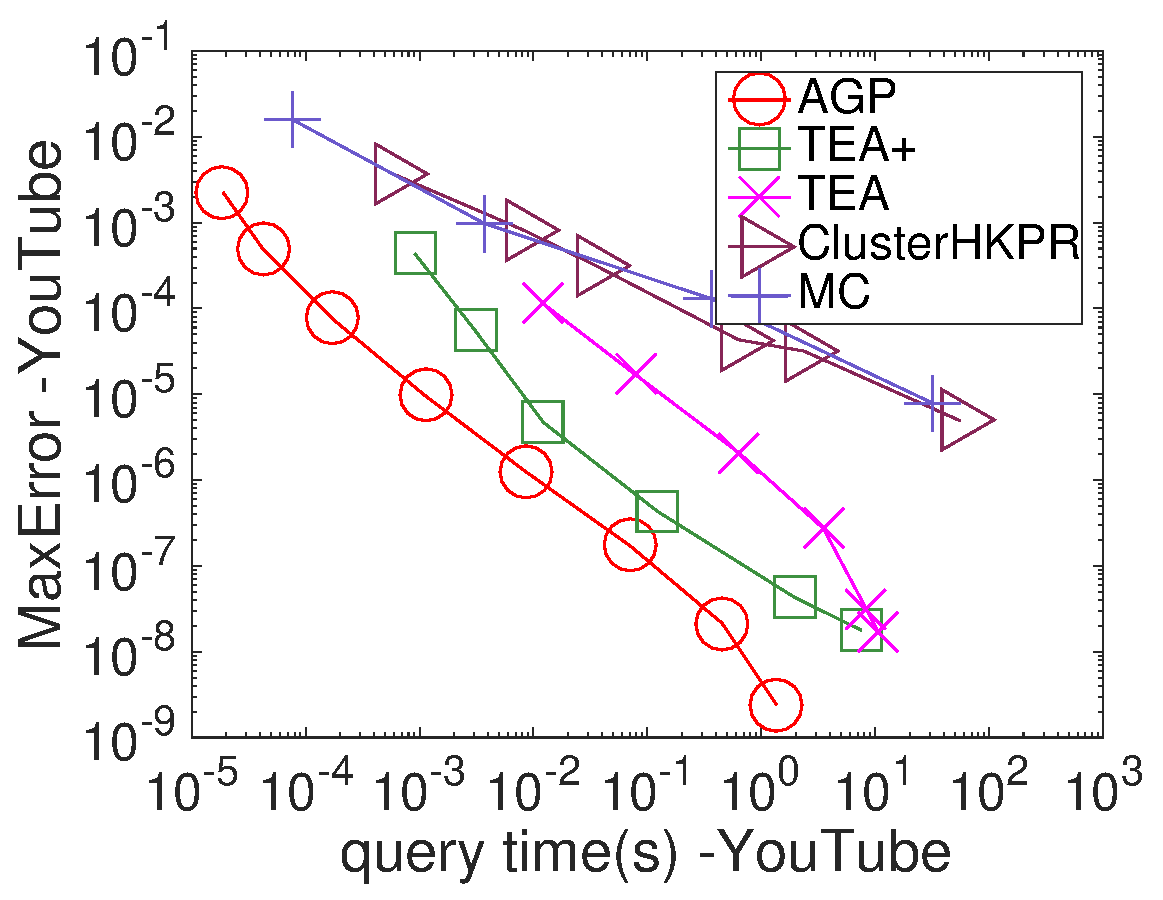
\includegraphics[height=34mm]{./Figs/HKPR-maxerr-query-YT.eps} &
			%\hspace{-3mm} 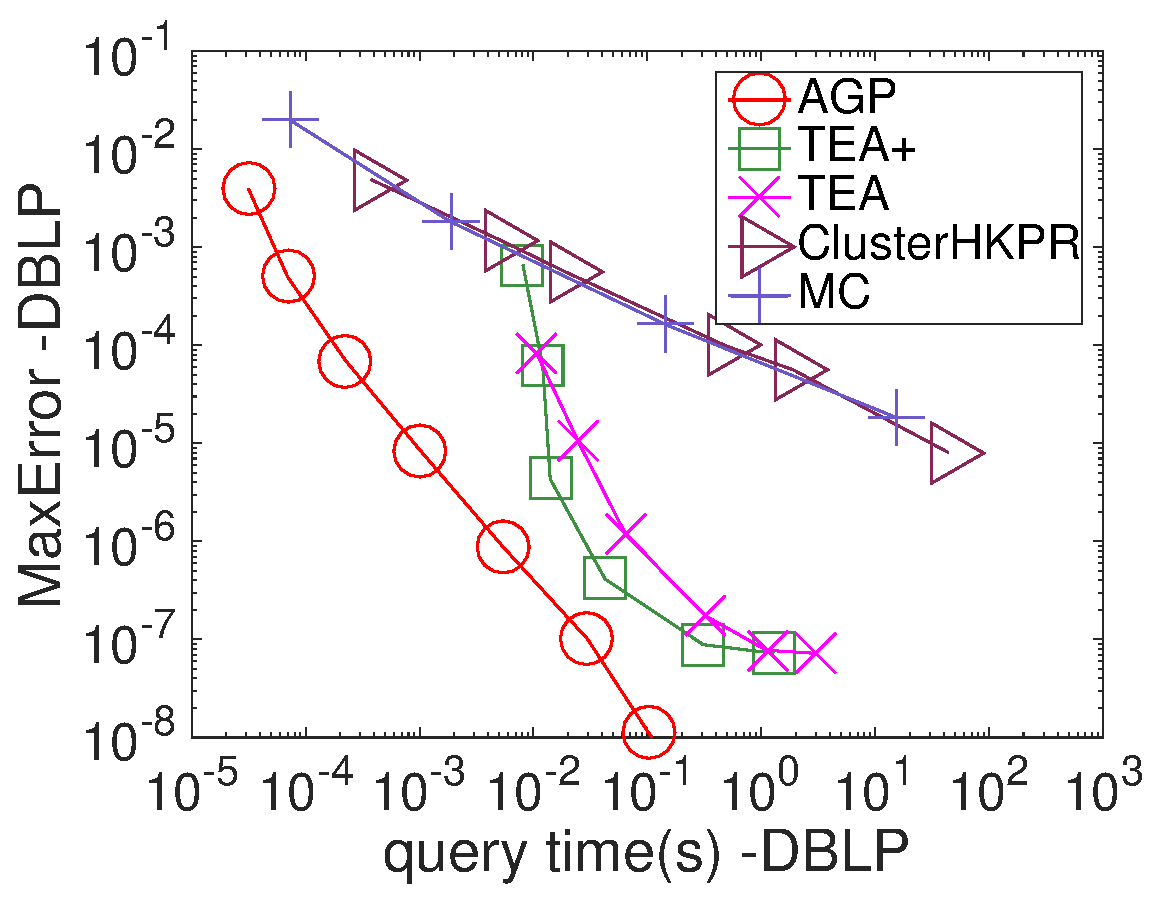
\includegraphics[height=25mm]{./Figs/HKPR-maxerr-query-DB.eps} &
			\hspace{-4mm} 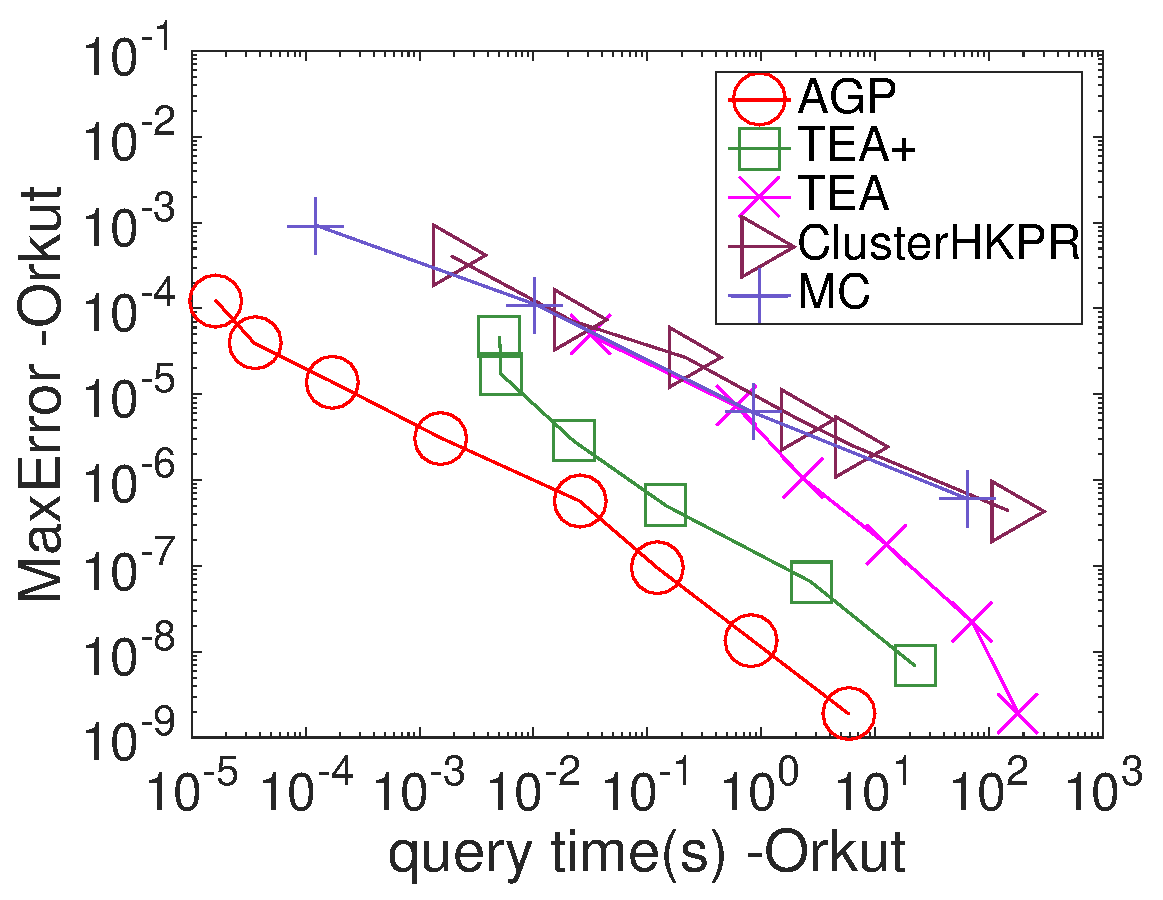
\includegraphics[height=34mm]{./Figs/HKPR-maxerr-query-OL.eps} &
			\hspace{-4mm} 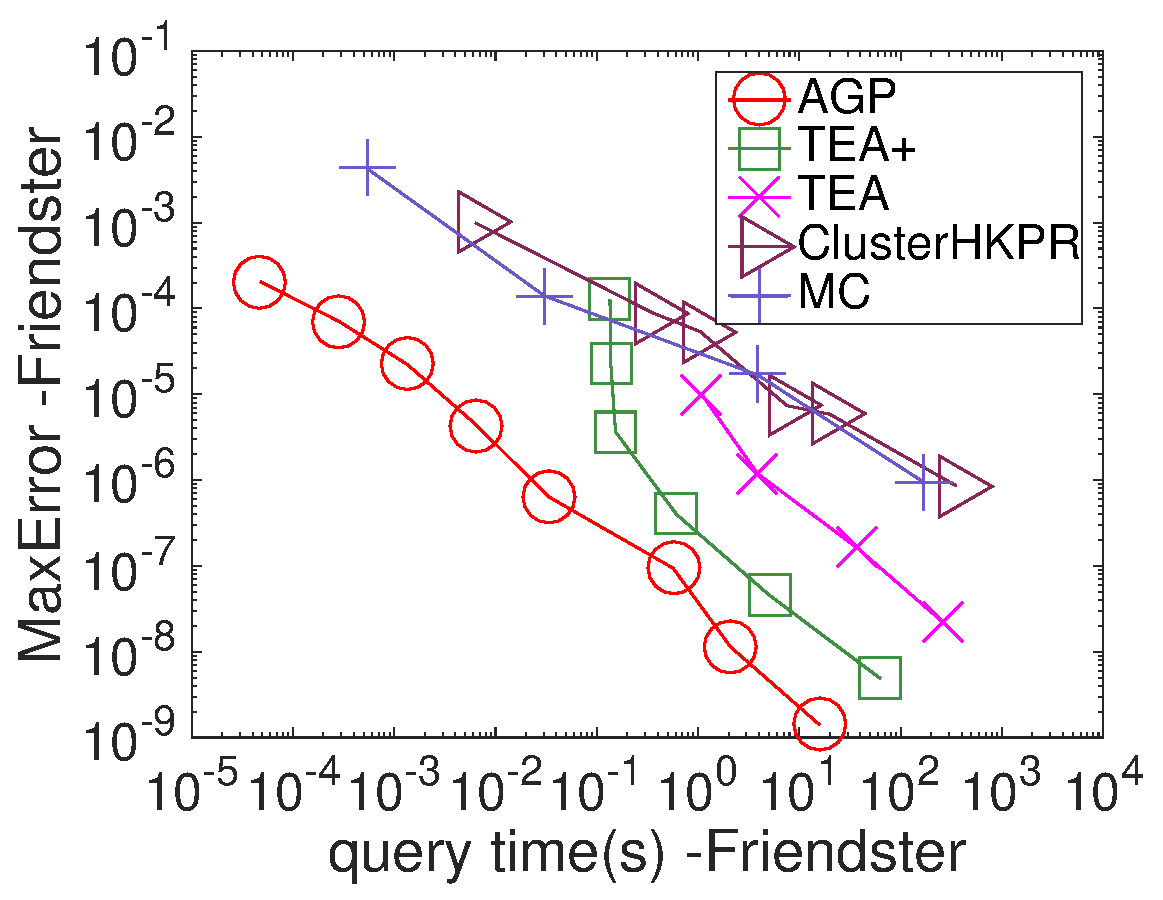
\includegraphics[height=34mm]{./Figs/HKPR-maxerr-query-FR.eps} &
			\hspace{-4mm} 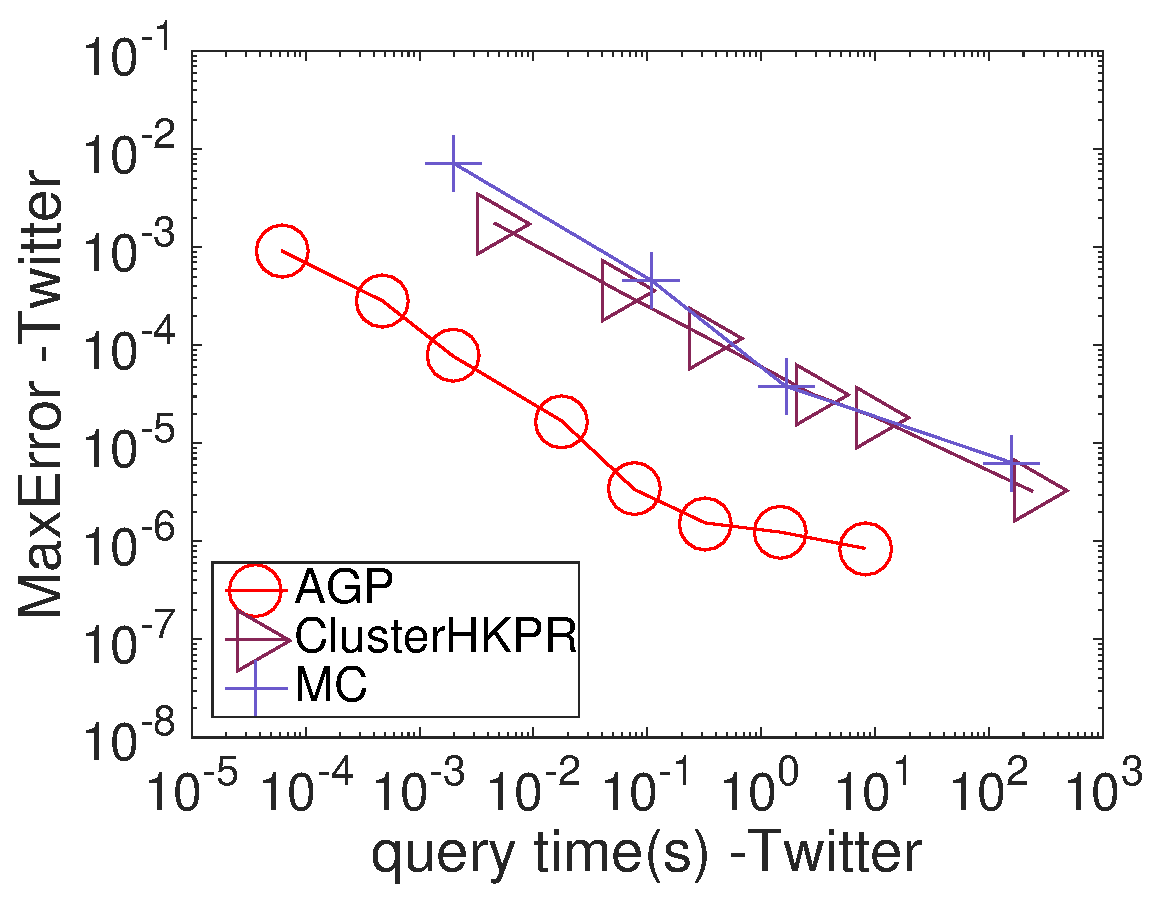
\includegraphics[height=34mm]{./Figs/HKPR-maxerr-query-TW.eps} 
		\end{tabular}
		\vspace{-5mm}
		\caption{Tradeoffs between {\em MaxError} and query time in local clustering.}
		\label{fig:HKPR-maxerror-query}
		\vspace{-2mm}
	\end{small}
\end{figure*}

\begin{figure}[t]
	\begin{small}
		\centering
		\vspace{-2mm}
		%    \begin{footnotesize}
		\begin{tabular}{cccc}
			%\multicolumn{4}{c}{\hspace{-4mm} \includegraphics[height=5mm]{./Figs/legend_large.eps}} \vspace{-1mm} \\
% 			\hspace{-2mm} 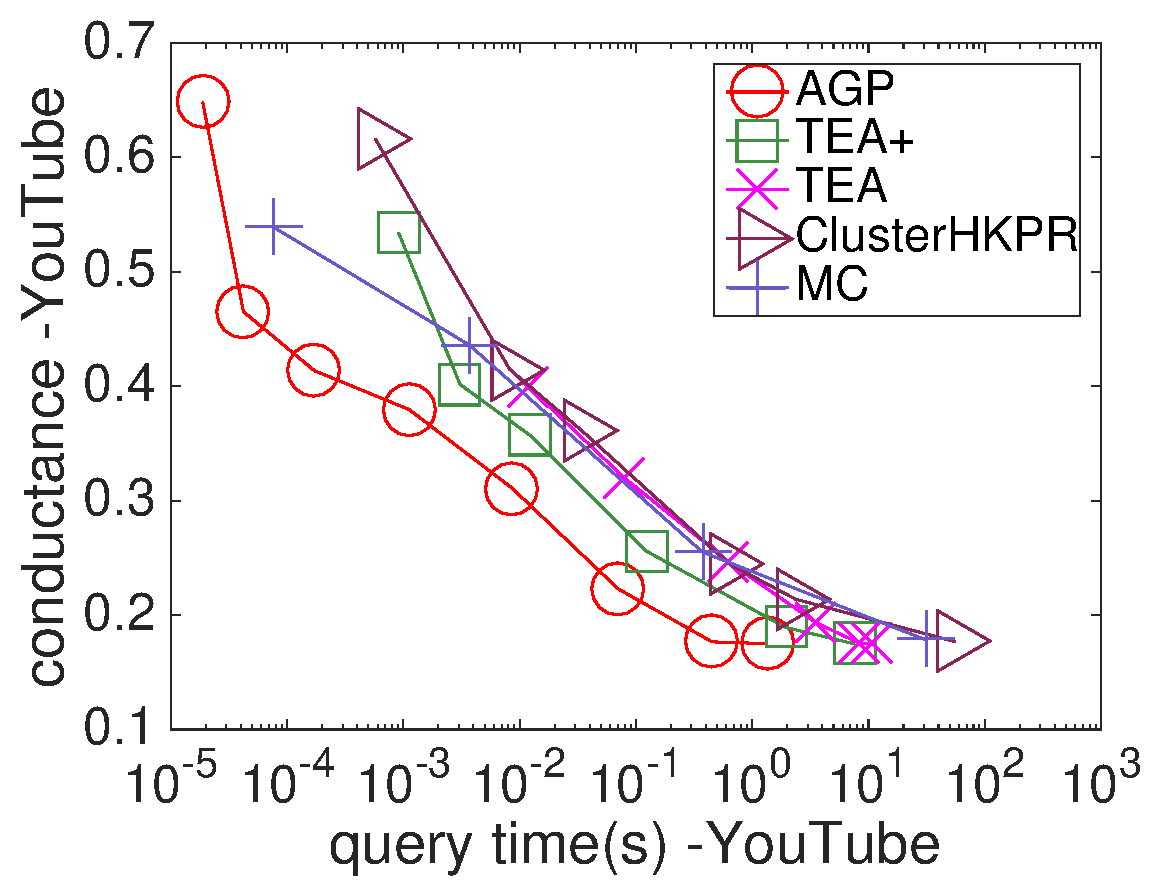
\includegraphics[height=34mm]{./Figs/HKPR-conductance-query-YT.eps} &
			%\hspace{-3mm} 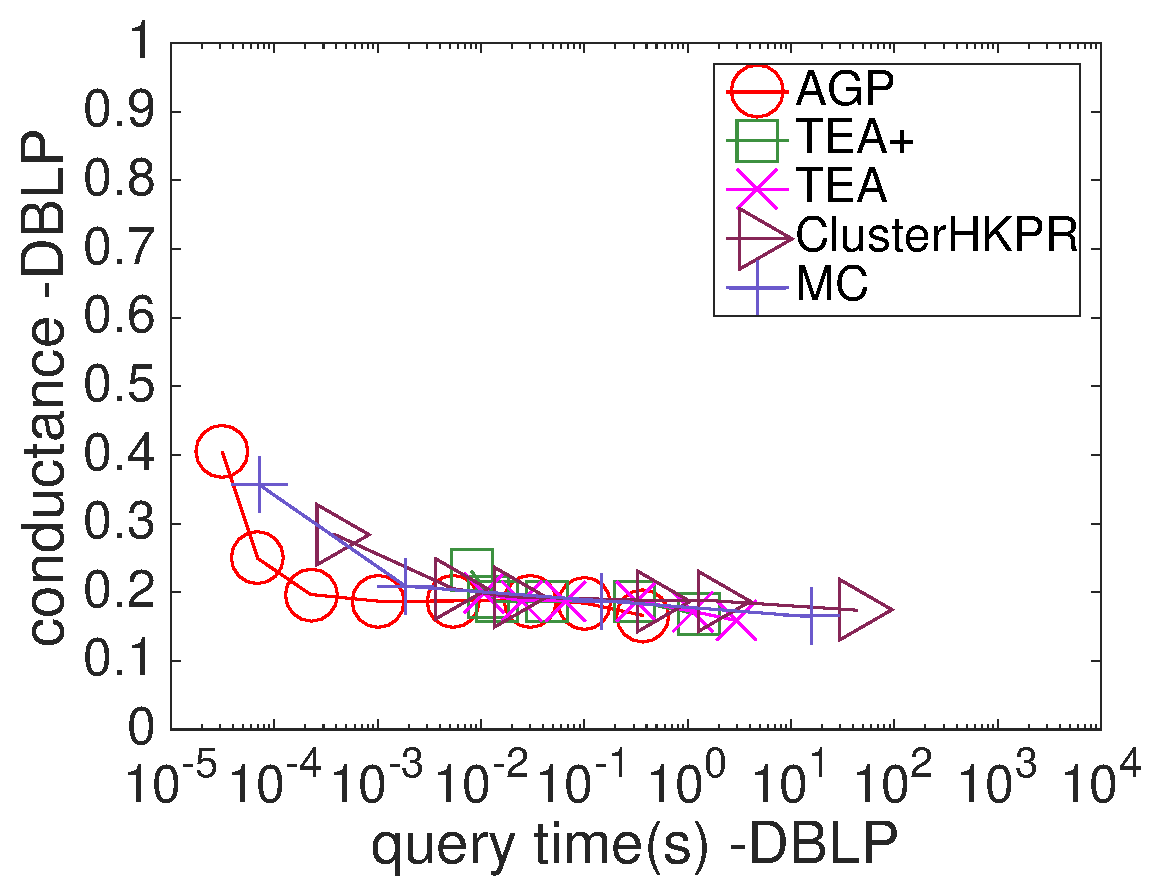
\includegraphics[height=25mm]{./Figs/HKPR-conductance-query-DB.eps} &
			\hspace{-4mm} 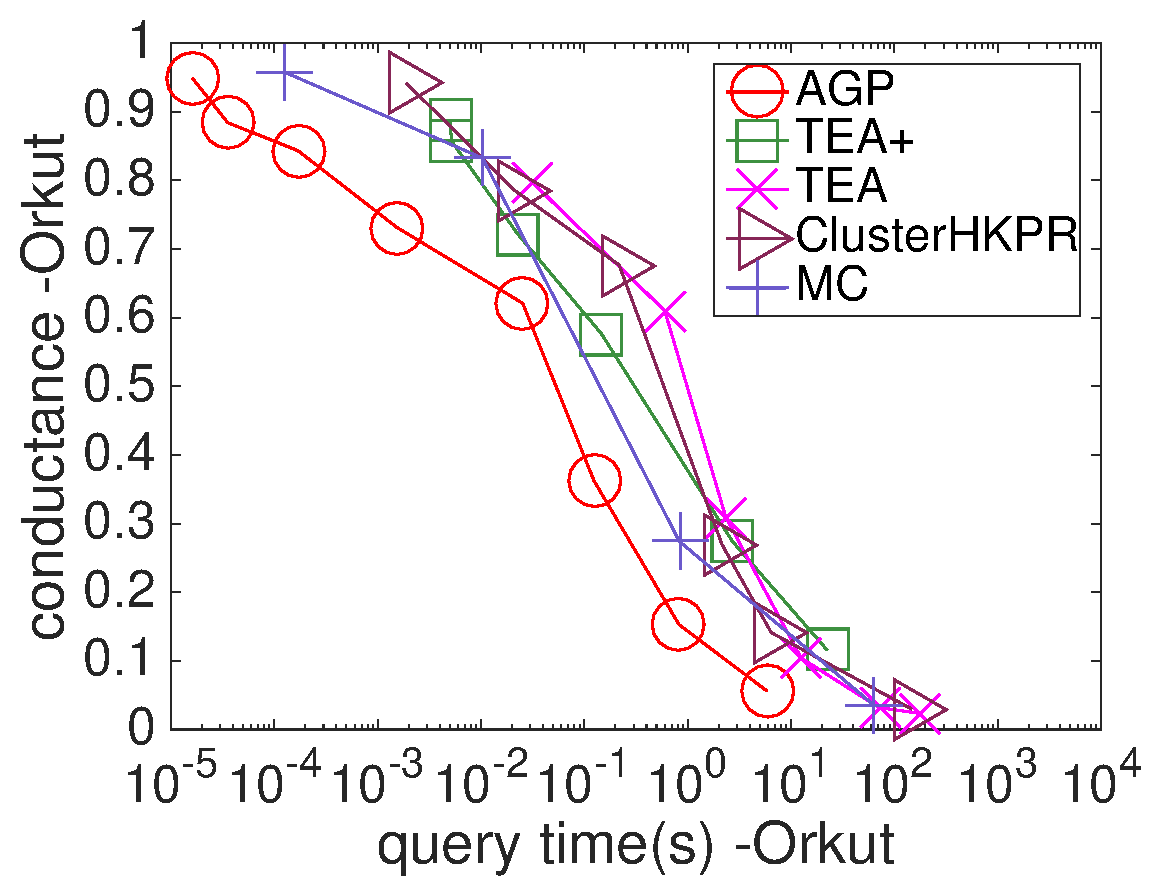
\includegraphics[height=32mm]{./Figs/HKPR-conductance-query-OL.eps} &
			\hspace{-4mm} 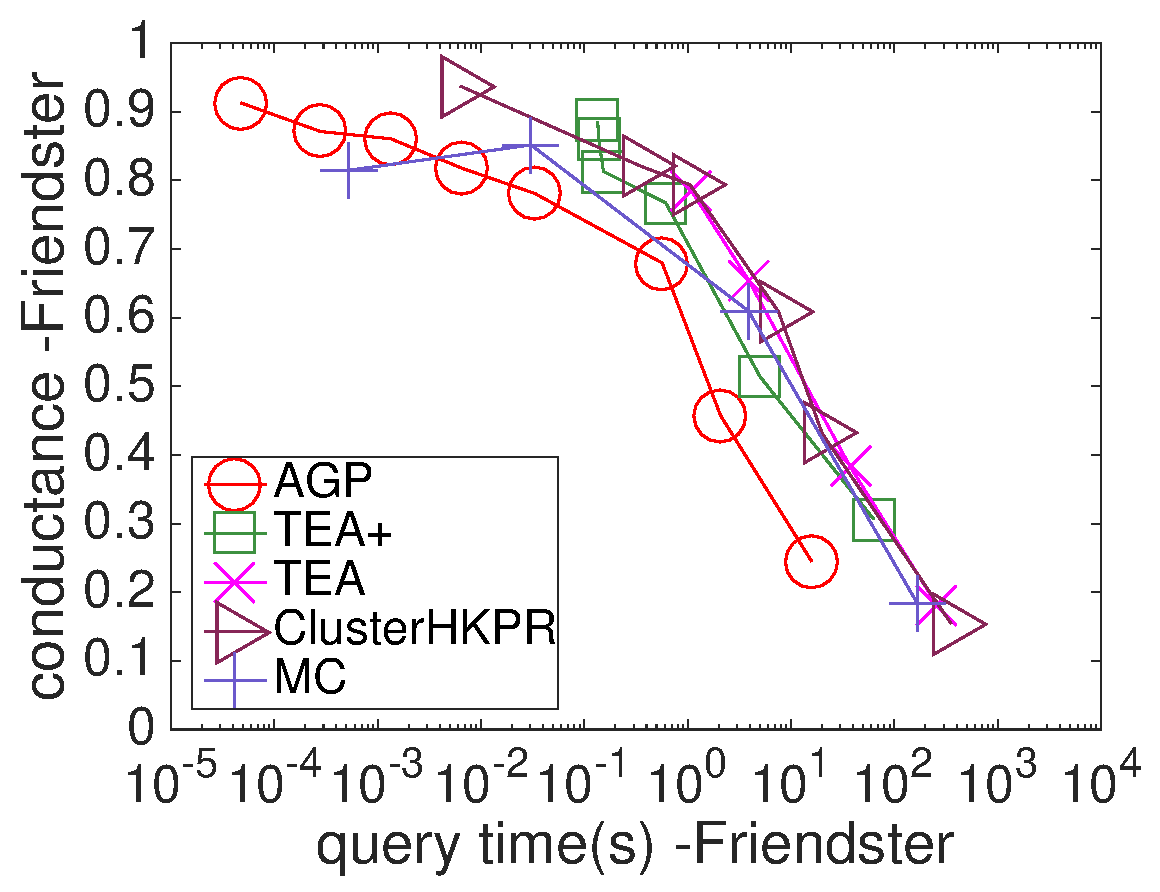
\includegraphics[height=32mm]{./Figs/HKPR-conductance-query-FR.eps} &
			%\hspace{-4mm} 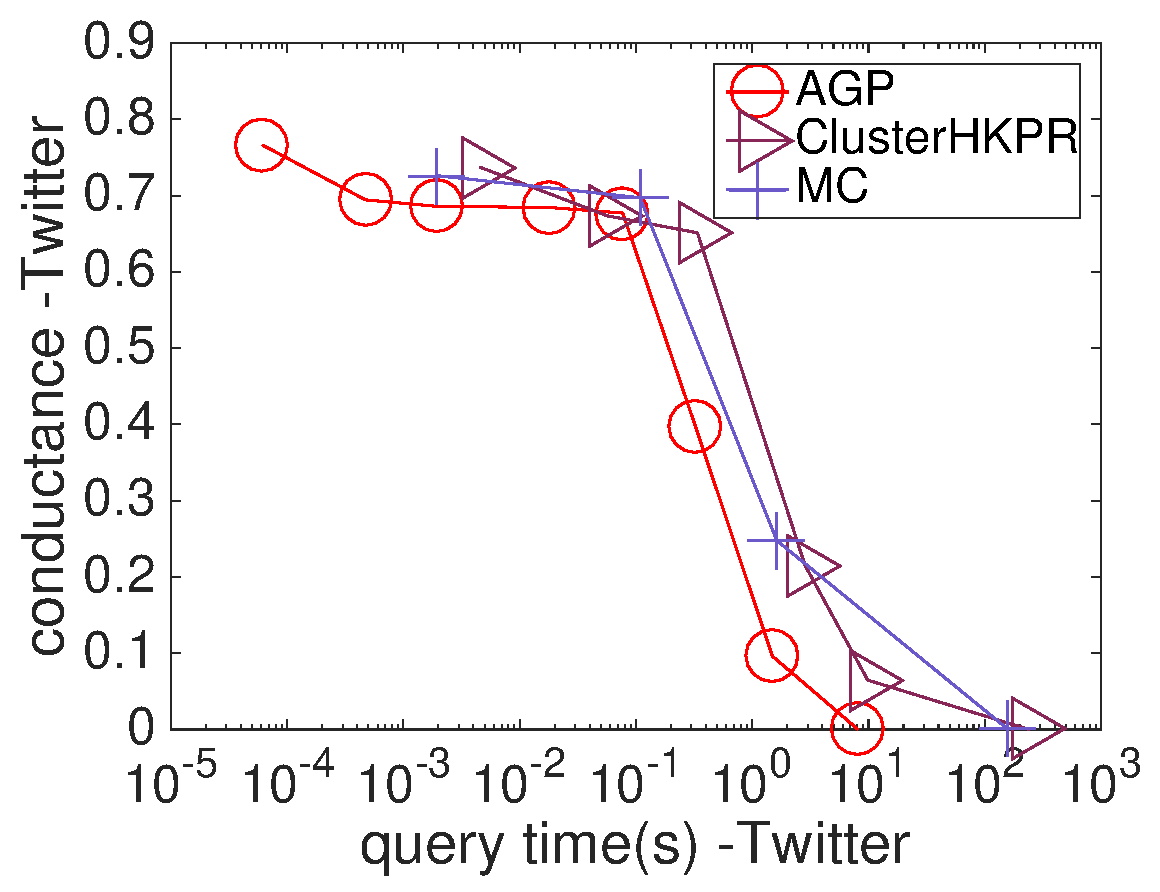
\includegraphics[height=34mm]{./Figs/HKPR-conductance-query-TW.eps} 
		\end{tabular}
		\vspace{-5mm}
		\caption{Tradeoffs between {\em conductance} and query time in local clustering.}
		\label{fig:HKPR-conductance-query}
		\vspace{-4mm}
	\end{small}
\end{figure}

In the next Lemma, we bound the variance of the approximate graph propagation vector $\hat{\pi}$, which takes a surprisingly simple form. 
\vspace{-1mm}
\begin{lemma}
\vspace{-1mm}
	\label{lem:variance}
    For any node $v \in V$, the variance of $\hat{\vec{\pi}}(v)$ obtained by Algorithm~\ref{alg:AGP-RQ} satisfies 
    %$	\Var \left[ \hat{\vec{\pi}}(v) \right]\le \frac{L(L+1)}{2} \cdot \varepsilon \cdot \vec{\pi}(v). $
    $	\Var \left[ \hat{\vec{\pi}}(v) \right]\le \frac{L(L+1)\varepsilon}{2} \cdot \vec{\pi}(v). $
    % \begin{equation}\nonumber
    % 	\begin{aligned}
    % 		\Var \left[ \hat{\vec{\pi}}(v) \right]\le \frac{L(L+1)}{2} \cdot \varepsilon \cdot \vec{\pi}(v). 
    % 	\end{aligned}
    % \end{equation}
\end{lemma}
\vspace{-1mm}
Recall that we can set $L=O(\log 1/\varepsilon)$ to obtain a relative error threshold of $\varepsilon$. Lemma~\ref{lem:variance} essentially states that the variance decreases linearly with the error parameter $\varepsilon$. Such property is desirable for bounding the relative error. In particular, for any node $v$ with $\vec{\pi}(v) > 100\cdot \frac{L(L+1)\varepsilon}{2}$, the standard deviation of $\hat{\vec{\pi}}(v)$ is bounded by ${1\over 10}\vec{\pi}(v)$. Therefore, we can set $\varepsilon = \delta \cdot \frac{200}{L(L+1)} = \Tilde{O}(\delta)$ and obtain the relative error guarantee in Definition~\ref{def:pro-relative}.
%implies that $\hat{\vec{\pi}}(v) - \vec{\pi}(v) \le  {1\over 10}\vec{\pi}(v)$ 
In particular, we have the following Theorem that bounds the expected cost of Algorithm~\ref{alg:AGP-RQ} under the relative error guarantee.

\vspace{-1mm}
\begin{theorem}\label{thm:RP-error}
Algorithm~\ref{alg:AGP-RQ} achieves an approximate propagation with relative error $\delta$, that is, for any node $v$ with $\vec{\pi}(v)>\delta$, $\left|\vec{\pi}(v)-\hat{\vec{\pi}}(v)\right|\hspace{-1mm} \leq \hspace{-1mm}\frac{1}{10} \cdot \vec{\pi}(v)$. The expected time cost can be bounded by
\vspace{-2mm}
\begin{equation*}
\vspace{-1mm}
E[Cost] =	O\left(\frac{L}{\delta}\cdot \sum_{i=1}^{L} \left\| Y_i \cdot \left(\mathbf{D}^{-a}\mathbf{A}\mathbf{D}^{-b} \right)^i \cdot \vec{x} \right\|_1\right).
\end{equation*}
\end{theorem}

To understand the time complexity in Theorem~\ref{thm:RP-error}, note that $ \left\| \left(\mathbf{D}^{-a}\mathbf{A}\mathbf{D}^{-b} \right)^i \cdot \vec{x} \right\|_1$ is the summation of the true residues at level $i$.  By the Pigeonhole principle, $ \frac{1}{\delta}\left\| Y_i \cdot \left(\mathbf{D}^{-a}\mathbf{A}\mathbf{D}^{-b} \right)^i \cdot \vec{x} \right\|_1$ is the upper bound of the residues at level $i$ that are larger than $\delta$. This bound is the output size of the propagation at level $i$, which means Algorithm~\ref{alg:AGP-RQ} achieves near optimal time complexity. 



Furthermore, we can compare the time complexity of Algorithm~\ref{alg:AGP-RQ} with other state-of-the-art algorithms in specific applications. For example, in the setting of heat kernel PageRank, the goal is to estimate $\vec{\pi}=\sum_{i=0}^\infty e^{-t} \cdot \frac{t^i}{i!}\cdot \left(\mathbf{A}\mathbf{D}^{-1} \right)^i \cdot \vec{e}_s $ for a given node $s$. The state-of-the-art algorithm TEA~\cite{yang2019TEA} computes an approximate HKPR vector $\hat{\vec{\pi}}$ such that for any $\pi(v)>\delta$, $|\vec{\pi}(v)-\hat{\vec{\pi}}(v)| \leq \frac{1}{10} \cdot \vec{\pi}(v)$ holds for high probability. By the fact that $t$ is the a constant and $\Tilde{O}$ is the Big-Oh notation ignoring log factors, the total cost of TEA is bounded by $O\left(t\log n \over \delta \right) = \Tilde{O}\left(1 \over \delta \right)$. On the other hand, in the setting of HKPR, the time complexity of Algorithm~\ref{alg:AGP-RQ} is bounded by 
\vspace{-2mm}
\begin{equation*}
\vspace{-2mm}
\frac{L}{\delta}\cdot \sum_{i=1}^{L} \left\| Y_i \cdot \left(\cdot \mathbf{A}^\top \mathbf{D}^{-1} \right)^i \cdot \vec{e}_s \right\|_1 = \frac{L}{\delta}\cdot \sum_{i=1}^{L} Y_i \le \frac{L^2}{\delta} = \Tilde{O}\left(1 \over \delta \right).
\end{equation*}
Here we use the facts that $ \left\| \left( \mathbf{A} \mathbf{D}^{-1} \right)^i \cdot \vec{e}_s \right\|_1 =1$ and $Y_i \le 1$. This implies that under the specific application of estimating HKPR, the time complexity of the more generalized  Algorithm~\ref{alg:AGP-RQ} is asymptotically the same as the complexity of TEA. Similar bounds also holds for Personalized PageRank and transition probabilities. We defer detailed explanation to the technical report~\cite{TechnicalReport}. 

	%For any $t \in V$ and $\ell \in \{0,1, 2, ... , L\}$, let $Z^{(\ell)}$ denote the term that:
%$$ Z^{(\ell)}(t)=\sum_{i=0}^{\ell-1} \frac{w_i}{Y_i}\hat{R}^{(i)}(t)+ \sum_{i=\ell}^{L}\sum_{u \in V} \frac{w_i}{Y_{\ell}} \cdot \hat{R}^{(\ell)}(u)\cdot p_{i-\ell}(u,t). $$
	 %The variance of $\hat{\pi}(t)$ obtained by Algorithm~\ref{alg:AGP-RQ} can be derived that:
    %\begin{align}\nonumber
    %	\Var \left[ \epi(t) \right]=\E \left[ \sum_{\ell=0}^{L-1}\Var \left[Z^{(\ell)}(t)\mid \hat{R}^{(0)},...,\hat{R}^{(\ell-1)}\right]\right]. 
    %\end{align}
		%Compute $p_{i+r_i} = \frac{1}{\delta}\cdot \frac{Y_{i+1}}{Y_i}\cdot \frac{\hat{\vec{r}}^{(i)}(u)}{d_{v_{i+r_i}}^a\cdot d_u^b}$ and add $v_{i+r_i}$ into $X$ with probability $\frac{p_{i+r_i}}{p_i}$\;\;
% consider the single-source PPR query from the source node $s$. Set $\delta=\frac{1}{n}$, which is commonly used in multiple applications. 
% $\vec{\hat{r}}^{(0)}(s)$ is initialized as $1$. $\vec{\hat{r}}^{(1)}(v_{1})=...=\vec{\hat{r}}^{(1)}(v_{n})=\frac{1-\alpha}{n}$ increased by the propagation from node $s$. Recall that the truncation rule asks to ignore all nodes with residues less than $\delta$. We need to abandon all propagations from node $v_{1},v_{1},...,$ and $v_{n}$ because $\vec{\hat{r}}^{(1)}(v_{j})=\frac{1-\alpha}{n}< \delta$ for $\forall j \in [1,n]$. Hence, $\hat{\vec{r}}^{(2)}(t)=0$ while the true value of residue $\vec{r}^{(2)}(t)=\left(1-\alpha\right)^2$. A large error can be caused by the simple truncation. 
%Simple truncation needs to be considered more efficiency. 
%So, truncate every nodes with small residues the trivial truncation leads to $\vec{\hat{r}}^{(2)}(t)=0$ and cause large error.  

% Indeed, consider the jump that start from neighbor $v_j$. The expectation of the geometric distributed random number $r$ is $1/p_j$, where $p_j$ is the probability of node $j$ being sampled. If $p_j$ is close to $0$, we may skip a large number of neighbors until the next sampled neighbor. 

% Actually, these is a sampling technique called {\em subset sampling} which can achieve independent sampling with small time cost. 
% We first illustrate the sampling process of subset sampling. Then we present the details to use subset sampling in our propagation structure. 
% %we conduct the sampling with the help of Sorted SubSet Sampling skill. 

% Considering an element set $S$, each element $x_i \in S$ has a pre-defined sampling probability $p_i$. The subset sampling problem wants to find an efficiency way to return the sample set, and guarantee each element $x_i \in S$ is sampled independently with the probability $p_i$. If we can pre-sort the elements $x_i \in S$ in the descending order of its sampling probability $p_i$, we call the problem as {\em sorted subset sampling}. 
% %To solve this problem, a naive method is to scan every element and check whether to be sampled one by one. We can guarantee independence of the sampling results by this naive way, while it's time cost is $O(|S|)$. If the sampling probability is relative small for the elements, $O(|S|)$ time cost can be much larger than the size of sampling results. 


% %As for the scenario that the sampling probability of each element is different, we can extend the above idea to further fix this problem. 

% Algorithm~\ref{alg:subsampling} extends the above idea for the scenario with different sampling probability. 
% %illustrates the pseudocode  to solve the Sorted SubSet Sampling problem. 
% Given the set $S$ of $h$ elements sorted by each element's sampling probability in the descending order, we initialize a variable $i$ as $0$, and a set $X$ as an empty set (Line 1). Then we repeat generating random numbers $r_i$ independently following the geometric distribution with parameter $p_i$ (Line 2-3). If $(i+r_i)$ does not exceed the number of elements $h$, we add the element $x_{i+r_i}$ to the set $X$ with probability $\frac{p_{i+r_i}}{p_i}$ (Line 4-6). Update $i$ as $(i+r_i)$ and move to the next iteration until $i$ exceeds $h$ (Line 7). After the process, we return the set $X$ as the sample set (Line 8). 
 
% %By theorem~\ref{thm:subsampling}, the Sorted Subset Sampling return the sample results efficiently and independently only if the sample elements sorted according to their sampling probability. 

% Note that the sorted subset sampling assumes all elements are sorted in the descending order of their sampling probability. In order to use sorted subset sampling in our propagation structure, we need to pre-sort the adjacency list of each node before the propagation process. Recall that for any node $u$ at level $i$, Algorithm~\ref{alg:AGP-RQ} samples the remained neighbors $v \in N_u$ with probability $p^{(i+1)}(u,v)=\frac{1}{\delta}\cdot \left(1-\frac{w_i}{Y_i} \right) \cdot \frac{\hat{R}^{(i)}(u)}{d_v^a\cdot d_u^b}$. Because the $d_u$ and $\hat{R}^{(i)}(u)$ are the same for every neighbor $v\in N_u$, we can sort the  adjacency list for $\forall v\in N_u$ only by $d_v$. The neighbors $\forall v\in N_u$ with large degrees correspond to small sampling probabilities.  
% % which is decreased by $d_v^a\cdot d_u^b$. Hence, we can pre-construct a sorted adjacency list for any node $u \in V$. 
% Thus we can append the neighbors $\forall v \in N_u$ to the adjacency list of $u$ by the ascending order of $d_v$. What's more, the sorting process can be finished in $O(m+n)$ time by counting sort, which asymptotically equals to the time cost of graph input. 

%Sorted Subset Sampling requires to sort every elements 


%As for the sampling process, a crucial point 
%In the sample process, if we check every neighbor to decide whether to sample, each propagation still cost $O(\bar{d})$, leading to the $O(m)$ cost for each iteration. 
%Hence, we adopt the techniques of subset sampling to finish the sample process during the time proportional to the size of the sampled set. 






%it asks to update the residue of all neighbors in every propagation operation, no matter how much the residue increases. 
%This costs $O(\bar{d})$ to touch every neighbor per propagation on average, where $\bar{d}$ denotes the average degree of the given graph. What's more, little residue can also increase the number of nodes with 





%\subsection{Subset Sampling}

 


%\subsection{Randomized Propagation}


% By this means, the number of nodes to be pushed in each iteration can be significantly  reduced. 
% Specifically, at each level $i\in [0,L-1]$, we pick the nodes $u$ to do the propagation only if $\hat{\vec{r}}^{(i)}(u)$ is larger than some threshold $\varepsilon$. By this means, the number of nodes to be pushed in each iteration can be significantly  reduced. 

%Moreover, note that in Algorithm~\ref{alg:AGP-deter}, the reserve $\hat{Q}^{(i)}(u)$ is only updated after the propagation from node $u$ at level $i$. If we decide not to do the propagation from node $u$
%Specifically, we can only pick the nodes $u$ satisfying $\left( 1- \frac{w_i}{Y_i}\right) \cdot \frac{\hat{R}^{(i)}(u)}{d_v^a\cdot d_u^b} \ge \delta$. Note that after the propagation from node $u$ at level $i$, for every neighbor $v\in N_u$, residue $\hat{R}^{(i+1)}(v)$ will be increased by $\left( 1- \frac{w_i}{Y_i}\right) \cdot \frac{\hat{R}^{(i)}(u)}{d_v^a\cdot d_u^b}$  according to the update rule. 

% To understand the variance bound of Algorithm~\ref{alg:AGP-RQ}, we observe that for each neighbor $v\in N_u$ with small degrees, we increase its residue by $\delta$ with probability $\frac{1}{\delta}\frac{Y_{i+1}}{Y_i} \cdot \frac{\hat{\vec{r}}^{(i)}(u)}{d_v^a\cdot d_u^b}$. Thus, the variance of this increment can be bounded by $ \delta^2\cdot \frac{1}{\delta}\frac{Y_{i+1}}{Y_i} \cdot \frac{\hat{\vec{r}}^{(i)}(u)}{d_v^a\cdot d_u^b} = \delta \cdot \frac{Y_{i+1}}{Y_i} \cdot \frac{\hat{\vec{r}}^{(i)}(u)}{d_v^a\cdot d_u^b} $. 

% for any node $u$ at level $i$, we transfer $\delta$ to its neighbors $v \in N_u$ with the probability $\frac{X^{(i+1)}(u,v)}{\delta}$. Thus, the variance of every propagation can be bounded by $\delta \cdot X^{(i+1)}(u,v)$. In each iteration from level $0$ to $L-1$,
% Meanwhile, the sum of residue increments totally received by nodes $v$ at level $i+1$ from its neighbors is $\vec{r}^{(i+1)}(v)=\sum_{u\in N_v} X^{(i+1)}(u,v)$. Hence, the variance of $\vec{r}^{(i+1)}(v)$ can be further bounded by $\delta \cdot \vec{r}^{(i+1)}(v)$. Sum up the variance of residues at the first $L$ levels. We can finally limit the variance of $\hat{\pi}(t)$ within $\delta \cdot \vec{\pi}(t)$ for every node $t \in V$, which is given in Lemma~\ref{lem:variance} in detail. 

% \begin{lemma}
% 	\label{lem:cost}
% 	The expected cost of Algorithm~\ref{alg:AGP-RQ} is bounded by
% 	\begin{align*}
% 	\E \left[Cost\right] \leq \frac{1}{\delta}\cdot \sum_{i=1}^{L} \left\| Y_i \cdot \left(\mathbf{D}^{-a}\cdot \mathbf{A}^\top \cdot \mathbf{D}^{-b} \right)^i \cdot \vec{x} \right\|_1.
% 	%\E \left[C_{total}\right] \leq \sum_{i=0}^{L-1} \sum_{v\in V} \frac{1}{\delta}\cdot R^{(i+1)}(v).
% 	\end{align*}
% \end{lemma}
% As for the total cost of Algorithm~\ref{alg:AGP-RQ}, we first consider the cost of one propagation, and sum them up in the end. For the propagation from node $u$ at level $i$ to its neighbor $v$, it will cost $1$ deterministically if $X^{(i+1)}(u,v)< \delta$, or with the probability $\frac{X^{(i+1)}(u,v)}{\delta}$ otherwise. Hence, the cost of one propagation can also be bounded by $\frac{X^{(i+1)}(u,v)}{\delta}$. Sum up all propagation for any node at the first levels. The total cost can be bounded by $\sum_{i=0}^{L-1}\sum_{v\in N_u} \frac{X^{(i+1)}(u,v)}{\delta}=\sum_{i=0}^{L-1} \frac{\vec{r}^{(i+1)}(v)}{\delta}$, which approximately equals the number of residues more than $\delta$ in the first levels. Recall that in Definition~\ref{def:pro-relative}, we want to estimate $\pi(t)$ precisely if $\pi(t)\ge \delta$. Thus, the number of residues more than $\delta$ is actually a lower bound of the propagation structure, and the cost of Algorithm~\ref{alg:AGP-RQ} achieves optimal asymptotically. 




% Finally, based on the three Lemma given above, we can derive Theorem~\ref{thm:RP-error}, which gives the error bound and time cost of our randomized propagation structure. 
%The proof of Theorem~\ref{thm:RP-error} can be divided into several parts given by the lemmas below. Lemma~\ref{lem:unbiasedness} first shows the unbiasedness of $\epi$. While Lemma~\ref{lem:variance} and Lemma~\ref{lem:cost} bound the variance and cost of $\epi$ derived by Algorithm~\ref{alg:AGP-RQ}. 




% \noindent{\bf Remarks.}



% we set the maximum level to do the propagation $L=\log{\frac{1}{\delta}}$ according to Assumption~\ref{asm:L} (Line 1). For each $i \in [0,L]$, initialize all vectors of $i$-hop residues and reserves as $\vec{0}$, except $\vec{\hat{r}}^{(0)}=\vec{x}$ (Line 2-3). In the iteration from level $0$ to $L-1$, we only deterministically do the propagation from the nodes $u$ to its neighbors $v\in N_u$, which satisfy $d_v^a\cdot d_u^b \hspace{-0.5mm} \le \hspace{-0.5mm} \frac{\hat{\vec{r}}^{(i)}(u)}{\delta} \cdot \frac{Y_{i+1}}{Y_i}$. 
% %In the propagation from node $u$ at level $i$ to its neighbor $v\in N_u$, 
% %For these node $u$ and their corresponding neighbors $v\in N_u$, 
% And increase $\hat{\vec{r}}^{(i+1)}(v)$ by $\frac{Y_{i+1}}{Y_i}\cdot \frac{\hat{\vec{r}}^{(i)}(u)}{d_v^a\cdot d_u^b}$ (Line 6-7). For the other neighbors $v \in N_u$, we sample them with the probability $\frac{1}{\delta}\cdot \frac{Y_{i+1}}{Y_i} \cdot \frac{\hat{\vec{r}}^{(i)}(u)}{d_v^a\cdot d_u^b}$ (Line 8-9). Then we transfer $\frac{w_i}{Y_i}\cdot \hat{\vec{r}}^{(i)}(u)$ to the reserve $\hat{\vec{q}}^{(i)}(u)$ and set $\hat{\vec{r}}^{(i)}(u)$ as $0$ (Line 10-11). After the $L_{th}$ iteration, return $\sum_{i=0}^L \hat{\vec{q}}^{(i)}$ as the estimation of $\pi$ (Line 12). 





% Again, we consider the toy graph in Figure~\ref{fig:special-case} and the task of estimating the 2-step transtion probability vector $\pi=\left(\mathbf{A} \cdot \mathbf{D}^{-1} \right)^2 \cdot \vec{e}_s $ from node $s$. As previously stated, to perform the propagation from $s$, we need to sample a small subset from $s$' neighbor set $N(s) = \{v_1, \ldots, v_n\}$.

% Even though each propagation received by node $t$ only brings quite small increments to its residue, a large number of propagations can accumulate these increments to a large residue.  


% Hence, other than truncate every propagation from the nodes with small residues, it's better to sample some neighbors to do the propagations. In detail, for each node $u \in V$ at level $i$ ($i\in [0,L-1]$), let $X^{(i+1)}(u,v)$ denote the residue increment of $\hat{\vec{r}}^{(i+1)}(v)$ caused by the propagation from node $u$ to its neighbor $v\in N_u$. 
% %For those propagations to some neighbors $v$ with small residue increment, such that 
% If $X^{(i+1)}(u,v)< \delta$, we can sample node $v$ with the probability $\frac{X^{(i+1)}(u,v)}{\delta}$ to determine whether propagating from node $u$ to $v$. Small residue increments correspond to small sampling probabilities. The sampling process only focus on the propagation with small residue increments. Thus, only a few number of sampling is expected to be conducted.  
% Thus, by this means, we can effectively avoid the error caused by the simple truncation without obviously extra time cost.
% %We can sample the neighbors to conduct the propagations 
% %it's better to truncate the propagation with small residue increments wisely, other than focus on nodes with small residues.
% %as for these propagation with little residue increments, we can use sampling to decide which to propagate, other than truncating these nodes trivially. 
% %Randomness can avoid the simple propagation truncation. 

% %Based on this idea, we propose a Randomized Propagation Algorithm, using randomness to avoid the large error caused by the truncated propagation. 


% Recall that we denote $X^{(i+1)}(u,v)$ as the increment of residue $\hat{\vec{r}}^{(i+1)}(v)$ caused by the propagation from node $u$ to $v$ ($v\in N_u$). By the recursive formula given in equation~\eqref{eqn:iteration}, $X^{(i+1)}(u,v)$ is expected to be $\frac{Y_{i+1}}{Y_i} \cdot \frac{\hat{\vec{r}}^{(i)}(u)}{d_v^a\cdot d_u^b}$. Algorithm~\ref{alg:AGP-RQ} deterministically do the propagation when this increment $X^{(i+1)}(u,v)$ is more than $\delta$, and use sampling to reduce the number of propagation with unbiasedness. 
%Note that in the propagation from node $u$ at level $i$ to its neighbor $\forall v\in N_u$, residue $\hat{R}^{(i+1)}(v)$ is expected to be increased by $\frac{Y_{i+1}}{Y_i} \cdot \frac{\hat{R}^{(i)}(u)}{d_v^a\cdot d_u^b}$  according to the update rule given in equation~\eqref{eqn:iteration}. 



% For ease of presentation, we first consider the simple case where $d_{v_1} = d_{v_2} = \ldots = d_{v_{d_v}}$. It follows that $p_1 = p_2= \ldots = p_{d_v}$. 


% If the sampling probability is identical for every element, denoting as $p$, we can generate a binomial random number $r\sim B(|S|,p)$ first. %$r$ tells us the number of elements to be sampled. 
% Then we generate $r$ uniform random numbers corresponding to the element ID to be sampled. In this way, we can finish the sampling process within the time $1+h$, where $h=|S|$. % denotes the number of elements in the element set $S$. 
% Moreover, we can further polish the sampling process by substituting geometric random number for the binomial random number. Denote a geometric random number $r_g\sim G(p)$, which means we need to go through $r_g-1$ failure before the first success. 
% Instead of using binomial random number to decide the number of sampling, it's better to repeat generating geometric random numbers to find the next element successfully sampled. We can save no less than 1 cost than to generate binomial random numbers. 



% for any node $u\in V$ at level $i$ ($i \in [0,L-1]$), we want to sample from those neighbors $v\in N_u$ to which whether propagating, when the residue increment $X^{(i+1)}(u,v)<\delta$. But if we check these candidate neighbors one by one, the time cost is equivalent to the power method actually. 
% %During the sample process, we aim to return the sample results with the time proportional to the size of the sample set. So we cannot scan every neighbor and decide whether to sample one by one. Otherwise, each propagation still cost $O(\bar{d})$, which is also a global propagation process and don't save time.
% % Wang et al.~\cite{wang2020RBS} propose a sampling technique to generate one random number for all neighbors. %They use the identical random number to sample every neighbor to be propagated. 
% %Though they can achieve a fast sampling with the time cost equals to the size of the sample set, every sampling is dependent for $\forall v\in N_u$. 
% How can we sample neighbors independently with the time cost proportional to the sample set? 

%With the help of sorted subset sampling, we can choose the neighbors independently without check every nodes meanwhile.

%%% Local Variables:
%%% mode: latex
%%% TeX-master: "paper"
%%% End:
